\chapter{UML-Klassendiagramme}
\renewcommand{\chaptertitle}{UML-Klassendiagramme}

\lehead[]{\normalfont\sffamily\hspace*{-2.00cm}\textcolor{white}{\colorbox{lightblue}{\makebox[1.60cm][r]{\thechapter}}}\hspace{0.17cm}\textcolor{lightblue}{\chaptertitle}}
\rohead[]{\textcolor{lightblue}{\chaptertitle}\normalfont\sffamily\hspace*{0.17cm}\textcolor{white}{\colorbox{lightblue}{\makebox[1.60cm][l]{\thechapter}}}\hspace{-2.00cm}}
%\chead[]{}
\rehead[]{\textcolor{lightblue}{AvHG, Inf, My}}
\lohead[]{\textcolor{lightblue}{AvHG, Inf, My}}

\lstset{style=myJava}

\section{Allgemeine Beziehungen: Assoziation}

Beispiel für die Beziehung zwischen der Klasse \myClass{Auto} und der Klasse
\myClass{Person}:

\begin{center}
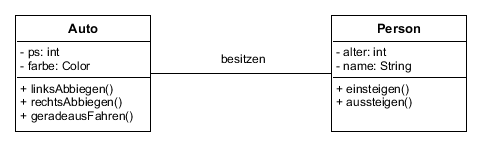
\includegraphics[width=0.8\textwidth]{./inf/SEKII/12_UML_Klassendiagramme/Assoziation.png}
\end{center}
% Hinweis an Autor: In Assoziation.png idealerweise Leserichtung ("wird gefahren von" oder Pfeil) ergänzen, 
% da Auto links und Person rechts steht.

Eine Beziehung zwischen zwei Klassen kennzeichnet man durch eine
Verbindungslinie. Über die Verbindungslinie schreibt man den Beziehungsnamen
(im Beispiel „besitzen“). Das UML-Fachwort für eine einfache Verbindung ist
\emph{Assoziation}.


\subsection{Multiplizität}

Die sogenannte Multiplizität gibt an, wie viele Objekte einer Klasse mit einem
Objekt der gegenüberliegenden Klasse verbunden sein können. Die Multiplizität
steht oberhalb der Verbindungslinie direkt neben der zugehörigen Klasse.

\subsubsection{Notation}

\begin{tabular}{lll}
1       & bedeutet & genau 1\\
1..4    & bedeutet & 1 bis 4\\
{}*     & bedeutet & beliebig viele (auch 0)\\
1..*    & bedeutet & beliebig viele, aber mindestens 1\\
\end{tabular}

\subsubsection{Beispiel}

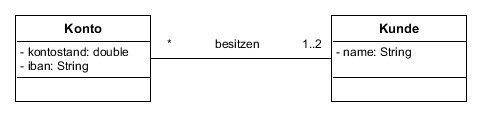
\includegraphics[width=0.8\textwidth]{./inf/SEKII/12_UML_Klassendiagramme/Multiplizitaet.png}

Die Angabe der Multiplizität ist folgendermaßen zu interpretieren:
Linke Seite: „Ein Kunde kann beliebig viele Konten besitzen (auch 0).“
Rechte Seite: „Jedes Konto gehört einer oder zwei Personen.“


\section{„Ist-Teil-von“-Beziehung: Aggregation}

\begin{minipage}{0.45\textwidth}
Sehr häufig sind „Ist-Teil-von“-Beziehungen.
Zum Beispiel sind Sitzplätze, Vorhang und
Bühne Teile eines Theaters. Ein anderes
Beispiel ist eine Adresse, die man in die
Bestandteile Name, Straße und Ortsangabe
zerlegen kann. Solche „Ist-Teil-von“-Beziehungen
bezeichnet man als \emph{Aggregation}.

Weil die „Ist-Teil-von“-Beziehung so häufig
vorkommt, gibt es für Aggregationen eine
spezielle Notation. Die Beziehungslinie wird an
der Seite des „Ganzen“ mit einer ungefüllten Raute
versehen.
\end{minipage}
\begin{minipage}{0.55\textwidth}
\begin{center}
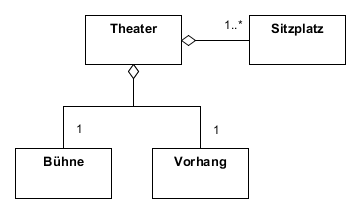
\includegraphics[width=0.9\textwidth]{./inf/SEKII/12_UML_Klassendiagramme/Aggregation.png}
\end{center}
\end{minipage}

\subsection{Komposition (starke Aggregation) \tagLK}

Eine besondere Form der Aggregation ist die \emph{Komposition}. Sie liegt vor, wenn die Teile 
existenzabhängig vom Ganzen sind -- das heißt, die Teile können ohne das Ganze nicht sinnvoll 
existieren und werden zusammen mit ihm erzeugt und gelöscht (z.\,B.\ Räume eines Gebäudes oder 
die Ziffern einer Digitaluhr). In UML wird eine Komposition durch eine \textbf{ausgefüllte Raute} 
auf der Seite des Ganzen dargestellt.


\section{„Ist-ein“-Beziehung: Vererbung}

\begin{minipage}{0.25\textwidth}
\begin{center}
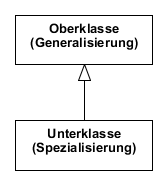
\includegraphics[width=0.9\textwidth]{./inf/SEKII/12_UML_Klassendiagramme/Vererbung.png}
\end{center}
\end{minipage}
\begin{minipage}{0.75\textwidth}
Häufig kommt es vor, dass eine Klasse einen Spezialfall einer anderen Klasse
darstellt. Z.\,B.\ sind die Klassen \myClass{Säugetier} und \myClass{Fisch} Spezialfälle der Klasse
\myClass{Tier}. Die Klassen \myClass{Löwe} und \myClass{Giraffe} sind wiederum Spezialisierungen der
Klasse \myClass{Säugetier}. Gleichzeitig sind sie natürlich auch Spezialisierungen der
darüberliegenden Klasse \myClass{Tier}. Zwischen der Spezialklasse und der
allgemeineren Klasse besteht also eine „Ist-ein“-Beziehung. In UML kennzeichnet
man eine solche Beziehung, indem man einen Pfeil mit nicht ausgefüllter Dreiecksspitze von der spezielleren Klasse zu
der allgemeineren Klasse zieht. Die spezielle Klasse bezeichnet man als
\emph{Unterklasse}, die allgemeine Klasse als \emph{Oberklasse}.
\end{minipage}

\clearpage

\subsection{Klassenhierarchie}

Beispiel für die \emph{Klassenhierarchie} der Tiere in einem Zoo:

\begin{center}
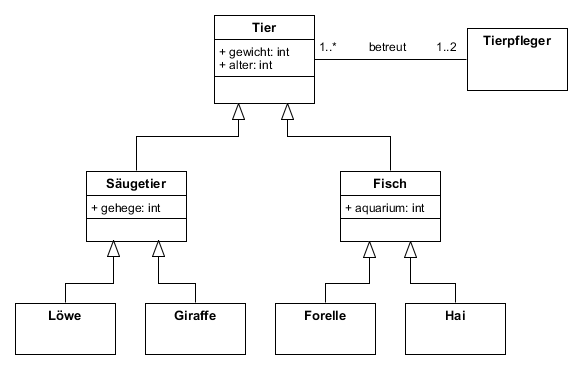
\includegraphics[width=0.8\textwidth]{./inf/SEKII/12_UML_Klassendiagramme/Zoo.png}
\end{center}
% Hinweis an Autor: Im Diagramm Zoo.png idealerweise die abstrakten Klassen (Tier, Säugetier, Fisch) kursiv setzen.

In der Oberklasse \myClass{Tier} sind alle Attribute, Methoden und Assoziationen
eingetragen, die für alle Tiere gemeinsam gelten. In den Unterklassen brauchen
diese gemeinsamen Eigenschaften nicht noch einmal eingetragen zu werden. In den
Unterklassen werden nur die Eigenschaften eingetragen, die für den
entsprechenden Spezialfall zutreffen. Z.\,B.\ besitzen alle Tiere ein Gewicht und
ein Alter. Jedes Tier wird von einem Tierpfleger betreut. Säugetiere und Fische
unterscheiden sich jedoch dadurch, dass sie in unterschiedlichen „Unterkünften“
leben. Ein Säugetier besitzt daher das zusätzliche Attribut \lstinline|gehege|, während
ein Fisch das Attribut \lstinline|aquarium| besitzt. Ein Löwe erbt von der Oberklasse
\myClass{Tier} die Attribute \lstinline|gewicht| und \lstinline|alter| sowie die Assoziation mit dem Tierpfleger.
Er besitzt auch das Attribut \lstinline|gehege|, das er durch seine direkte Oberklasse
\myClass{Säugetier} erbt. Ein Löwe hat jedoch nicht das Attribut \lstinline|aquarium|, da er kein
Fisch ist.

Da Attribute, Methoden und Beziehungen von der Oberklasse an die Unterklasse
vererbt werden, bezeichnet man „Ist-ein“-Beziehungen auch als
\emph{Vererbungsbeziehungen}.


\subsection{Abstrakte Klassen}

Ein UML-Diagramm wird dadurch übersichtlich, dass man die Gemeinsamkeiten von
verschiedenen Klassen in Oberklassen zusammenfasst. Häufig gibt es jedoch
keine konkreten Objekte von den angelegten Oberklassen. In dem Zoo-Beispiel
gibt es z.\,B.\ kein konkretes Objekt der Klasse \myClass{Säugetier}, weil die konkreten Objekte
immer den spezielleren Klassen \myClass{Löwe}, \myClass{Giraffe} usw.\ zugeordnet werden
müssen. Wenn keine konkreten Objekte für eine Oberklasse existieren können,
sagt man, die Klasse sei \emph{abstrakt}.

In UML-Klassendiagrammen erkennt man abstrakte Klassen daran, dass der Klassenname
\emph{kursiv} geschrieben wird (alternativ steht unter dem Klassennamen der Zusatz 
\lstinline|{abstract}|).
